\documentclass[12pt,letterpaper]{article}
\usepackage[utf8]{inputenc}
\usepackage[spanish]{babel}
\usepackage{amsmath}
\usepackage{amsfonts}
\usepackage{amssymb}
\usepackage{natbib}
\usepackage{graphicx}
\usepackage{cite}
\usepackage{wrapfig}
\usepackage{afterpage}
\setcitestyle{square}
\usepackage[export]{adjustbox}
\usepackage[left=2cm,right=2cm,top=2cm,bottom=2cm]{geometry}
\usepackage{afterpage}
\usepackage{setspace}
\spanishdecimal{.}
\usepackage{hyperref}
\usepackage{float}

\author{C. Iván Pineda S.\textsuperscript{1} }
\title{Trabajo final:"Caja" de herramientas, explicación de su uso.\\ Taller de Modelación Numérica}
\date {\textit{\textsuperscript{1}Universidad Nacional Autónoma de México}
\\ 5 de junio de 2018}

\begin{document}
\maketitle

Para correr el programa solo es necesario escribir en la terminal de linux  "python main.py", es necesario tener las librerias de numpy, matplotlib, mpl\_toolkits y math, normalmente vienen incluídas con la instalación de anaconda.

Posteriormente se empezarán a pedir desde la terminal los datos necesarios para resolver la ecuación, no es necesario mover nada de código, todo se solicita paso a paso desde la terminal (Fig. \ref{fig:ejemplo}).

\begin{figure}[H]
	\begin{center}
		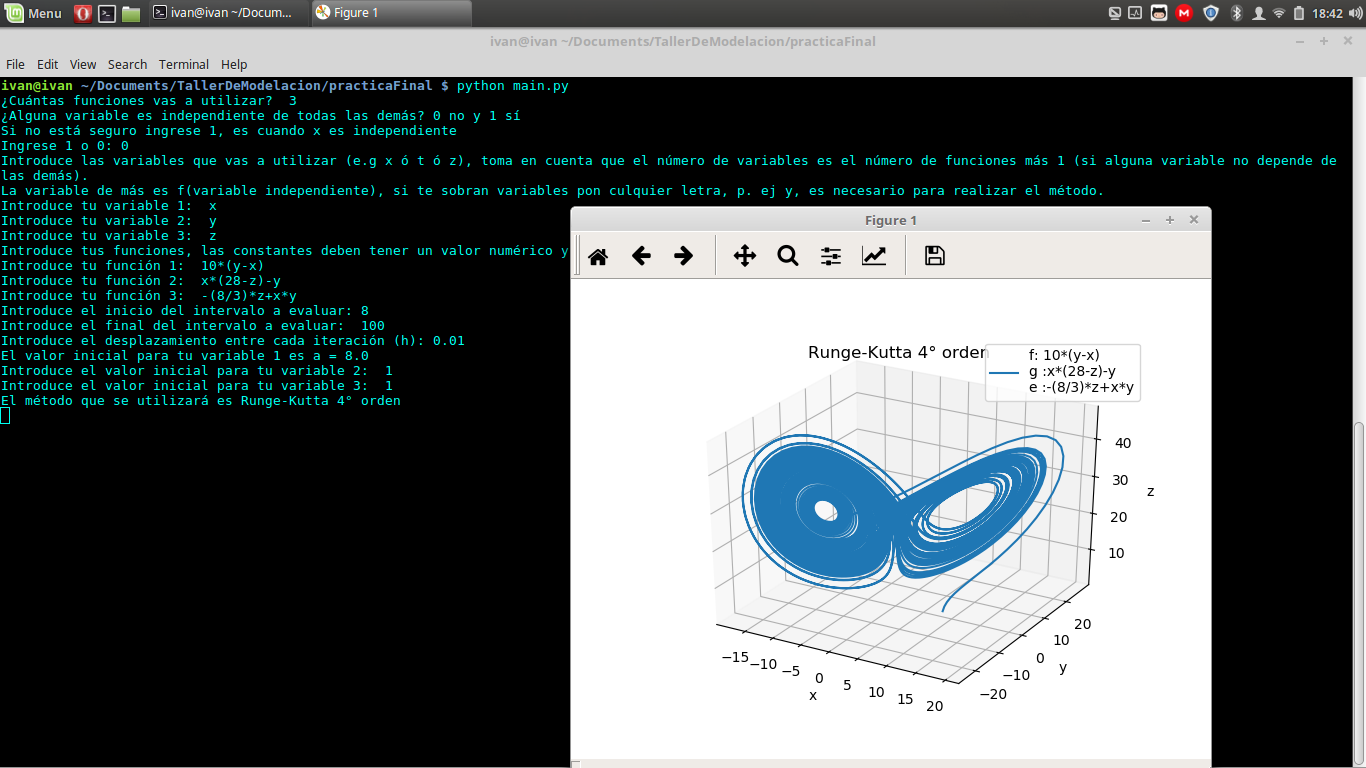
\includegraphics[scale=0.36]{3drk} 
	\end{center}
	\caption{Ejemplo de uso del programa y visualización de la gráfica obtenida.}
	\label{fig:ejemplo}
\end{figure}

En la carpeta de EjemplosDeUso vienen más ejemplos como el de la imágen.


\end{document}

